	\documentclass[10pt,oneside]{CBFT_book}
	% Algunos paquetes
	\usepackage{amssymb}
	\usepackage{amsmath}
	\usepackage{graphicx}
	\usepackage{libertine}
% 	\usepackage[bold-style=TeX]{unicode-math}
	\usepackage{lipsum}

	\usepackage{natbib}
	\setcitestyle{square}

	\usepackage{polyglossia}
	\setdefaultlanguage{spanish}
	



	\usepackage{CBFT.estilo} % Cargo la hoja de estilo

	% Tipografías
	% \setromanfont[Mapping=tex-text]{Linux Libertine O}
	% \setsansfont[Mapping=tex-text]{DejaVu Sans}
	% \setmonofont[Mapping=tex-text]{DejaVu Sans Mono}

	%===================================================================
	%	DOCUMENTO PROPIAMENTE DICHO
	%===================================================================

\begin{document}

% =================================================================================================
\chapter{Conceptos fundamentales de electromagnetismo}
% =================================================================================================


% =================================================================================================
% \section{Ecuaciones de Maxwell}
% =================================================================================================

La idea del curso es resolver las ecuaciones que describen matemáticamente el comportamiento clásico 
de los campos electromagnéticos, es decir las ecuaciones de Maxwell, en diversas situaciones.
Luego, la conexión con la fuerza que experimentarán las partículas cargadas por la acción de dichos
campos vendrá descripta por la fuerza de Lorentz.

Panorámicamente, lo dicho corresponde a trabajar con el set de ecuaciones
\[
	\divem{D} = 4 \pi \rho_\ell \qquad \divem{B} = 0 
\]
\[
	\rotorm{E} = - \frac{1}{c} \dpar{\vb{B}}{t} 
	\qquad 
	\rotorm{H} = \frac{4\pi}{c} \vb{J}_\ell + \frac{1}{c}\dpar{\vb{D}}{t},
\]
las cuales permiten determinar a los campos $\vb{E}, \vb{D}, \vb{B}, \vb{H}$ a partir de la densidad 
de carga $\rho$ y de corriente $\vb{J}$ (notemos que también los campos $\vb{D}$ y $\vb{B}$ influyen
en el comportamiento de $\vb{H}$ y $\vb{E}$).
Finalmente, la fuerza de Lorentz que actúa sobre una partícula de carga $q$ que se mueve con velocidad
$\vb{v}$ es
\[
	\vb{F} = q \left( \vb{E} + \frac{1}{c} \pv{v}{B} \right).
\]

Crudamente podemos decir que de esto trata el electromagnetismo clásico.
Las ecuaciones de Maxwell son lineales, de modo que vale la superposición aunque los campos tienen en
sí matemáticamente naturaleza diferente.
Los campo $\vb{E}, \vb{D}$ don ejemplos de vectores polares (aquellos que tienen bien definido el sentido,
como la fuerza, la posición y la velocidad) mientras que $\vb{B}, \vb{H}$ son ejemplos de vectores axiales,
que por el contrario tienen su sentido definido por una convención, como por ejemplo las velocidades
angulares.

De acuerdo con ello, el carácter de vector axial o polar tiene consecuencias en la transformación de
los mismos. Las transformaciones que se considerarán serán rotaciones, reflexiones espaciales y reflexiones
temporales. Las ecuaciones de Maxwell permanecen invariantes ante estas transformaciones.

\notamargen{Si multiplico vectorialmente dos vectores polares obtengo un vector axial.}

% Son ecuaciones lineales de modo que vale la superposición (con \vb{E}, \vb{B} y 
% cualquier vector relacionado linealmente con ellos).

El resto del capítulo recorrerá lo que es la construcción usual del electromagnetismo; primeramente considerar 
situaciones estáticas, independientes del tiempo, lo cual hace que aparezcan como fenómenos independientes la 
electricidad y el magnetismo y luego repasar someramente algunas propiedades matemáticas útiles para el
formalismo.

% =================================================================================================
\section{Electrostática}
% =================================================================================================

La ley de Coulomb establece que 
\[
	\vb{F}_{12} = k \: q_1 q_2 \frac{(\vb{x}_1 - \vb{x}_2)}{|\vb{x}_1 - \vb{x}_2 |^3}
\]
es la fuerza sobre la partícula en $\vb{x}_1$ debido a la partícula en $\vb{x}_1$. La constante $k$ está para ajustar
las unidades. En sistema gaussiano es $k=1$ y adimensional.
La Figura \ref{fig_ft1_ejescargas} ilustra la situación para el caso en que ambas cargas tienen igual signo; en ese
caso la fuerza $\vb{F}_{12}$ tiene la dirección del vector $\vb{x}_1 - \vb{x}_2$: apunta desde la fuente hacia el punto 
donde se evalúa.

\begin{figure}[!h]
	\begin{center}
	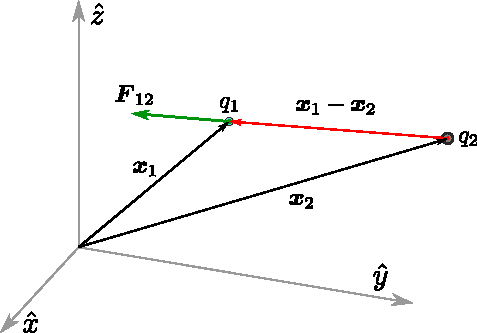
\includegraphics[width=0.5\textwidth]{images/fig_ft1_ejescargas.pdf}	 
	\end{center}
	\caption{Fuerza sobre la carga $q_1$ debida a la carga $q_2$.}
	\label{fig_ft1_ejescargas}
\end{figure} 

Cuando la carga $q_1$ es suficientemente pequeña como para no perturbar a la carga $q_2$ que origina la fuerza, se puede 
utilizar la ley de Coulomb para definir el campo eléctrico según
\[
	\vb{E}_{12}(\vb{x}_1) \equiv \lim_{q_1 \to 0} \frac{\vb{F}_{12}}{q_1}.
\]

Para una distribución discreta de $N$ cargas $q_i$ y tomando $\vb{x}_1 \equiv \vb{x}$ se tiene
\[
	\vb{E}(\vb{x}) = \sum_{i=1}^N \; q_i \frac{(\vb{x} - \vb{x}_i)}{|\vb{x} - \vb{x}_i |^3}.
\]
En el límite en que las cargas están lo suficientemente próximas como para considerar que forman se tiene una distribución
de carga de volumen $\rho(\vb{x})$, la expresión del campo adopta la forma de una integral
\[
	\vb{E}(\vb{x}) = \int_{V'} \rho(\vb{x}') \frac{(\vb{x} - \vb{x}')}{|\vb{x} - \vb{x}' |^3} \: dV' 
\]
donde $V'$ es el volumen de integración. En general \vb{x} es el llamdo punto campo y $\vb{x}'$ punto fuente.

\subsection{Conservación de la carga}

Aceptaremos el principio de conservación de la carga; la carga eléctrica no se genera ni se destruye. 
Considerando una región $\Omega$ en el espacio (cuya frontera está fija) la carga total encerrada en la
misma es 
\[
	Q(t) = \int_\Omega \rho(\vb{x}',t)\: d\Omega,
\]
siendo su variación temporal 
\[
	\dtot{Q(t)}{t} = \int_\Omega \dpar{\rho(\vb{x}',t)}{t} \: d\Omega,
\]
donde la derivada total se transforma en una derivada parcial debido a que el volumen es fijo.
\notamargen{Acá creo que la derivada debería ser la parcial desde el vamos. Check!}

La conservación de la carga nos dice que como la carga no aparece ni desaparece mágicamente, entonces
la variación de la carga contenida en $\Omega$ en cualquier instante de tiempo se debe al flujo neto de 
carga de la misma; es decir a la diferencia entre la que abandona la región y aquella que entra.
Como ilustra esquemáticamente la Figura \ref{conserv_carga}, la variación de carga $\Delta Q$ en un
dado $\Delta t$ corresponde a la diferencia entre las entrantes y las salientes.

La forma que tiene ese flujo se construye a partir del análisis ilustrado en el inserto de la figura.
Allí se ve un elemento pequeño $\delta \Omega$ que linda con la frontera de la región. Este elemento
$\delta V$ es lo suficientemente pequeño como para que en su interior el campo de velocidad de
las cargas sea constante. La {\it caja} $\delta V$ tiene un volumen que se puede expresar $\ell \delta S$
(longitud de la caja por área de la base). La longitud $\ell $ se elige como
$ \ell = v_n \delta t$, donde $v_n$ es la componente de la velocidad normal a la superficie. Así elegido, 
el volumen $\delta V = v_n \delta t \delta S$ representa el volumen que pasaría a través de $\delta S$ 
en el tiempo $\delta t$. En efecto, la partícula más lejana del borde $\delta S$ que está a distancia $\ell$ 
recorrerá en $\delta t$ justamente esa distancia (la velocidad $v$ es constante para todo el elemento).
Si la velocidad estuviese orientada hacia adentro, entonces tendríamos un bloque similar de carga 
entrante, y el razonamiento es el mismo.

La cantidad de carga $\delta Q$ que atraviesa el área $\delta S$ será entonces 
\[
	\delta Q = \rho \delta V = \rho v_n \delta S \delta t = \rho \vb{v} \cdot (\hat{n} \delta S) \delta t
\]
donde se ha expandido la velocidad normal. Entonces la variación de la carga en el elemento es
\[
	\frac{\delta Q}{\delta t} = \rho \vb{v} \cdot (\hat{n} \delta S).
\]

Si el producto escalar entre la velocidad y la normal es positivo entonces esto significa que la carga
abandona la superficie mientras que el caso contrario implica carga entrando en la misma. Entonces 
debemos ajustar la expresión anterior con un signo menos. Entonces, pasando al continuo
\[
	\dpar{Q}{t} = - \int_{\partial\Omega} \: \vb{J} \cdot d\vb{S}
\]
donde $\vb{J} = \rho \vb{v}$ es el vector densidad de corriente y $d\vb{S} = \hat{n}dS$ es el diferencial
de superficie vectorial.

Entonces, juntando las dos expresiones para la carga tenemos 
\[
	\int_\Omega \dpar{\rho(\vb{x}',t)}{t} \: d\Omega = - \int_{\partial\Omega} \: \vb{J} \cdot d\vb{S},
\]
y aplicando el teorema de la divergencia en el miembro derecho
\[
	\int_\Omega \dpar{\rho(\vb{x}',t)}{t} \: d\Omega = - \int_\Omega \: \divem{J} \: d\Omega,
\]
o bien 
\[
	\int_\Omega \left[ \dpar{\rho(\vb{x}',t)}{t} + \divem{J} \right] \: d\Omega = 0,
\]
y como esto vale para cualquier volumen $\Omega$ se sigue que el corchete debe ser nulo, de modo que se tiene
\[
	\dpar{\rho}{t} + \divem{J} = 0,
\]
que es la ecuación de continuidad de la carga.

% Entonces la carga que existe en una región depende de la tasa con la cual entra a la misma y aquella con la que la abandona.
% La carga total sale de una integral 
% \[
% 	Q = \int_{V'}  \rho(\vb{x}') dV'
% \]
% como muestra la imagen
\begin{figure}[htb]
	\begin{center}
	\includegraphics[width=0.25\textwidth]{images/fig_ft1_conserv.pdf}	 
	\end{center}
	\caption{}
	\label{conserv_carga}
\end{figure} 
% y si el volumen es fijo podemos tomar la derivada con respecto al tiempo que pasa el interior como
% derivada parcial,
% \[
% 	\dtot{Q}{t} = \int_{V'} \dpar{\rho}{t} (\vb{x}') dV' = - \int_{S\equiv\partial V'} \vb{J} \cdot d\vb{S}
% \]
% y el miembro extremo derecho  se debe a que si la carga varía es a consecuencia de que se va en
% forma de flujo. 
% Aplicando el teorema de la divergencia en el miembro derecho,
% \[
% 	\int_{V'} \dpar{\rho}{t} (\vb{x}') dV' = - \int_{V'} \nabla \cdot \vb{J} \; dV'
% \]
% lo cual vale para todo volumen y entonces esto significa que
% \[
% 	\dpar{\rho}{t} + \nabla \cdot \vb{J} = 0
% \]
% que es la ecuación de continuidad de la carga. 
\notamargen{Si fuera $\nabla \cdot \vb{J}=0$ esto significa que las líneas
de \vb{J} no tienen principio ni fin.Check!}

Si es $\divem{J}=0$ no se acumula carga; las líneas de $\vb{J}$ no tienen principio ni fin.
Los problemas de corrientes estacionarias cumplen esta condición. Esta condición en la ecuación de continuidad
nos dice que la distribución de carga no varía con el tiempo.

% =================================================================================================
\section{Interacción magnética}
% =================================================================================================

Cuando se da $\nabla \cdot \vb{J}=0$ hablamos de una corriente estacionaria (no hay acumulación de carga en
ninguna parte). Las corrientes estacionarias producen efectos magnéticos dados por la ley de Biot-Savart
\[
	\vb{B}(\vb{x}) = \frac{1}{c} \int_\Gamma \frac{I d\vb{\ell}' \times (\vb{x} - \vb{x}')}{|\vb{x} - \vb{x}'|^3} 
\]
que es válida para un circuito $\Gamma$, que es una curva que se recorre en sentido CCW.
En el caso de un volumen la expresión es 
\[
	\vb{B}(\vb{x}) = \frac{1}{c} \int_{V'} \frac{ \vb{J}(\vb{x}') \times (\vb{x} - \vb{x}')}{|\vb{x} - \vb{x}'|^3} 
dV'
\]
mientras que la fuerza sobre un circuito $\Gamma$ es
\[
	F = \frac{1}{c} \int_\Gamma I d\vb{\ell} \times \vb{B}
\]
y sobre un volumen 
\[
	F = \frac{1}{c} \int_V \vb{J} \times \vb{B} dV
\]

La transformación entre estas integrales puede hacerse merced al siguiente razonamiento,
% \begin{align*}
%  	I d\vb{\ell} \times \vb{B} = \vb{J}  \cdot d\vb{S} d\vb{\ell}  \times \vb{B} =
%   	\cos(\theta) dS \vb{J} d\ell \times \vb{B} = \\
% 	\vb{J} \times \vb{B}  \cos(\theta) dS d\ell  = \vb{J} \times \vb{B}  d\vb{S} \cdot d\vb{\ell}  = 
% 	\vb{J} \times \vb{B}  dV 
% \end{align*}
\[
  	I d\vb{\ell} \times \vb{B} = \vb{J}  \cdot d\vb{S} d\vb{\ell}  \times \vb{B} =
  	\cos(\theta) dS \vb{J} d\ell \times \vb{B} = 
\]
\[
	\vb{J} \times \vb{B}  \cos(\theta) dS d\ell  = \vb{J} \times \vb{B}  d\vb{S} \cdot d\vb{\ell}  = 
	\vb{J} \times \vb{B}  dV 
\]

\subsection{Fuerza de un circuito sobre otro}

La fuerza de un circuito 2 sobre otro circuito 1 puede calcularse con un poco de paciencia como sigue
\[
	F_{12} = \frac{1}{c} \int_{\Gamma_1} I_1 d\vb{\ell}_1 \times \left\{
	\frac{1}{c} \int_{\Gamma_2} \frac{I_2 d\vb{\ell}_2 \times (\vb{x}_1 - \vb{x}_2)}{|\vb{x}_1 - \vb{x}_2|^3} 
	\right\}
\]
\[
	F_{12} = \frac{I_1 I_2}{c^2} \int_{\Gamma_1} \int_{\Gamma_2} d\vb{\ell}_1 \times \left\{
	\frac{d\vb{\ell}_2 \times (\vb{x}_1 - \vb{x}_2)}{|\vb{x}_1 - \vb{x}_2|^3} 
	\right\}
\]
\[
	F_{12} = \frac{I_1 I_2}{c^2} \int_{\Gamma_1} \int_{\Gamma_2} d\vb{\ell}_2  \left\{
	\frac{d\vb{\ell}_1 \cdot (\vb{x}_1 - \vb{x}_2)}{|\vb{x}_1 - \vb{x}_2|^3} 
	\right\} - \int_{\Gamma_1} \int_{\Gamma_2} \frac{ (\vb{x}_1 - \vb{x}_2)}{|\vb{x}_1 - \vb{x}_2|^3} 
	\left\{ d\vb{\ell}_1 \cdot d\vb{\ell}_2 \right\}
\]
donde el primer término se comprueba nulo si se reescribe utilizando que
\[
	\frac{ (\vb{x}_1 - \vb{x}_2)}{|\vb{x}_1 - \vb{x}_2|^3} = 
	\nabla_{\vb{x}_2} \frac{ 1 }{|\vb{x}_1 - \vb{x}_2|} =
	- \nabla_{\vb{x}_1} \frac{ 1 }{|\vb{x}_1 - \vb{x}_2|} 
\]
de manera que entonces
\[
	- \int_{\Gamma_2} d\vb{\ell}_2  \int_{\Gamma_1} d\vb{\ell}_1 \cdot \nabla_{\vb{x}_1} \frac{ 1 }{|\vb{x}_1 - \vb{x}_2|} 
\]
donde se ve que es nula la última integral dado que 
\[
	\int_{\Gamma_1} d\vb{\ell}_1 \cdot \nabla_{\vb{x}_1} = 0.
\]

Entonces, se tiene 
\[
	F_{12} = - \frac{I_1 I_2}{c^2} \int_{\Gamma_1} \int_{\Gamma_2} \frac{ (\vb{x}_1 - \vb{x}_2)}{|\vb{x}_1 - \vb{x}_2|^3} 
	\left( d\vb{\ell}_1 \cdot d\vb{\ell}_2 \right)
\]
que vale lo mismo si intercambiamos $\Gamma_1$ con $\Gamma_2$ en la integración. Podemos decir que con corrientes estacionarias
vale el principio de acción y reacción: las fuerzas son iguales y de sentido opuesto.


% =================================================================================================
\section{Teorema de Helmholtz}
% =================================================================================================

Nos dice que un campo vectorial está completamente determinado por su divergencia y su rotor.
Por ejemplo, para un campo eléctrico 
\[
	\vb{E} = \int_{V'} \rho \frac{\vb{x} - \vb{x}'}{|\vb{x} - \vb{x}'|^3} dV' = 
		- \int_{V'} \rho \nabla_{\vb{x}} \frac{ 1 }{|\vb{x} - \vb{x}'|} dV' = 
		- \nabla_{\vb{x}} \int_{V'}   \frac{ \rho }{|\vb{x} - \vb{x}'|} dV' = 
\]
y esta última es la integral de Poisson
\[
	\vb{E} = - \nabla_{\vb{x}} \phi (\vb{x}).
\]
Entonces $\vb{E}$ es un gradiente y por ello 
\[
	\nabla  \times \vb{E} = 0
\]
de manera que $\vb{E}$ es conservativo, cumple $\int \vb{E}\cdot d\vb{\ell} = 0$ o lo que
es lo mismo, $\vb{E}$ es irrotacional.
Hemos hecho la construcción de un potencial electrostático.

% =================================================================================================
\section{Ley de Gauss}
% =================================================================================================



\begin{figure}[htb]
	\begin{center}
	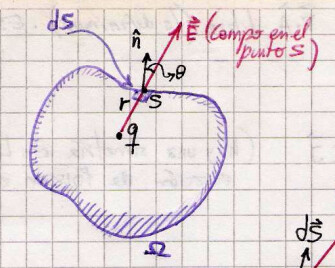
\includegraphics[width=0.35\textwidth]{images/fig_ft1_gauss.pdf}	 
	\end{center}
	\caption{}
\end{figure} 
\[
	\vb{E} \cdot \hat{n} = q \frac{\cos(\theta)}{r^2}
\]
y el ángulo sólido es
\[
	\vb{E} \cdot \hat{n} dS = q \frac{\cos(\theta)}{r^2} dS
\]
\[
	\vb{E} \cdot \hat{n} dS = q d\Omega \qquad \longrightarrow \qquad 
	\int_{S\equiv\partial V} \vb{E} \cdot \hat{n} \; dS = q \int_S d\Omega =
	\begin{cases}
	 0 \quad \textrm{carga exterior}\\
	 4\pi \quad \textrm{carga interior}
	\end{cases}
\]
\[
	\int_S \vb{E} \cdot \hat{n} \; dS = 4\pi \sum_i q_i
\]
La ley de Gauss es
\[
	\int_S \vb{E} \cdot \hat{n} \; dS = 4\pi Q_n
\]
donde $Q_n$ es la carga neta dentro de la superficie $S$. Al continuo pasa como 
\[
	\int_S \vb{E} \cdot \hat{n} \; dS = 4\pi \int_V \rho \: dV
\]
de manera que 
\[
	\int_V \divem{E} \; dV = \int_V 4\pi \rho \: dV
\]
y entonces
\[
	\divem{E} = 4\pi \rho.
\]

Por otro lado si \vb{E} es el gradiente de un potencial $\phi$ se tiene
\[
	\divem{E} = \Nabla\cdot{(-\Nabla\phi)} = - \lapm\phi = 4\pi \rho
\]
y se desprenden las ecuaciones de Poisson,
\[
	\lapm\phi = -4\pi \rho
\]
y de Laplace
\[
	\lapm\phi = 0
\]
que es el caso particular de la anterior con cargas nulas.

La solución de la ecuación no homogénea es suma de una solución del homogéneo más una solución
particular. La carga está relacionada a la solución particular.

\subsection{Gauges}

Dado que $\divem{B}=0$ entonces existe un \vb{A} tal que 
\[
	\rotorm{A} = \vb{B}
\]
pero para caracterizar totalmente el \vb{A} tengo la libertad de definir a conveniencia
\[
	\divem{A} \equiv \; \textrm{``el gauge''}.
\]
Casos particulares importantes son el gauge de Coulomb,
\[
	\divem{A} = 0
\]
de manera que como 
\[
	\Nabla \times (\rotorm{A}) = \Nabla(\divem{A}) - \lapm{\vb{A}} = \frac{4\pi}{c}\vb{J}
\]
se llega para el potencial electromagnético, bajo el gauge de Coulomb, a que 
\[
	\lapm{\vb{A}} = - \frac{4\pi}{c}\vb{J} 
\]

	\begin{table}[hbt]
	\centering
        \begin{tabular}{|c|c|}
		\hline
		& \\
		$\displaystyle{\vb{E} = \int_{V'} \frac{\rho(\vb{x}')(\vb{x}-\vb{x}')}{|\vb{x}-\vb{x}'|^3} dV' 
		}$ & $\displaystyle{\vb{B} = \frac{1}{c} \int_{V'} \frac{\vb{J}(\vb{x}') \times 
		(\vb{x}-\vb{x}')}{|\vb{x}-\vb{x}'|^3} dV'}$ \\
		& \\
		\hline
		Ley de Gauss & Ley de Ampere \\
		& \\
		$\displaystyle{\int_S \vb{E}\cdot d\vb{S} = 4\pi Q_n}$ &
		$\displaystyle{\int_\Gamma \vb{B}\cdot d\vb{\ell} = \frac{4\pi}{c} I_c}$ \\
		& \\
		\hline
		&\\
		$\divem{E} = 4\pi\rho$ & $\divem{B} = 0$ \\
		$\rotorm{E} = 0$ & $\rotorm{B} = \frac{4\pi}{c}\vb{J}$ \\
		& \\
		\hline
		& \\
		$\vb{E} = - \Nabla\phi$ & $\vb{B} = \rotorm{A}$ \\
		& \\
		\hline
        \end{tabular} 
	\caption{}
	\end{table} 

La operación de tomar rotor y el producto vecrtorial cambian el carácter de los vectores: de
polares pasan a axiales y viceversa.

La fuerza general sobre una distribución de carga es
\[
	\vb{F} = \int_{V'} \rho \vb{E} dV' + \frac{1}{c} \int_{V'} \vb{J} \times \vb{B} dV'. 
\]

\subsection{Delta de Dirac}

Una densidad de carga puntual se puede escribir mediante una delta de Dirac de acuerdo a
\[
	\rho(\vb{x}') = q\: \delta (\vb{x} - \vb{x}') = \begin{cases}
	                                               0 \qquad \vb{x} \neq \vb{x}' \\
	                                               \infty \qquad \vb{x} = \vb{x}'\\
	                                              \end{cases}
\]
siendo las dimensiones de la delta las de $1/L^3$ y cumpliéndose 
\[
	\int_{V'} \delta (\vb{x} - \vb{x}') dV' = 1
\]
\[
	\delta (\vb{x} - \vb{x}') = \frac{1}{h_1h_2h_3} \delta(q_1-q_1') \delta(q_2-q_2') \delta(q_3-q_3')
\]
donde $q_1, q_2$ y $q_3$ son coordenadas curvilíneas generales y $h_1h_2h_3$ es el jacobiano
de la transformación.
Luego
\[
	\int f(\vb{x}) \delta' (\vb{x} - \vb{x}_0) dx = -f'(\vb{x}_0)
\]



\subsection{reflexión}

Un vector polar sufre reflexión especular mientras que un vector axial ({\it pseudovector})
sufre una antireflexión especular. Ver la figura.

\begin{figure}[htb]
	\begin{center}
	\includegraphics[width=0.6\textwidth]{images/fig_ft1_reflexvect.pdf}	 
	\end{center}
	\caption{}
\end{figure} 

Una reflexión más una rotación permite eliminar componentes de campo.
Una simetría más una rotación-traslación permite eliminar dependencias.

Lo primero que debe hacerse es escribir bien la \vb{J} a partir del dato de la corriente
(que es el que se suele tener) mediante
\[
	i = \int_S \vb{J} \cdot d \vb{S}
\]
En cambio, para \vb{A} es más fácil usar
\[
	\vb{B} = \rotorm{A}
\]
y despejar de aquí la ecuación diferencial que emplear
\[
	\vb{A} = \frac{1}{c} \int_V \frac{\vb{J}}{|\vb{x}-\vb{x}'|} dV
\]


\section{El potencial vector}

Por la ley de Biot y Savart,
\[
	\vb{B} = \frac{1}{c} \int_{V'} \frac{\vb{J}(\vb{x}') \times (\vb{x}-\vb{x}')}{|\vb{x}-\vb{x}'|^3} 
	dV' = \Nabla_x \times \frac{1}{c} \int_{V'} \frac{\vb{J}(\vb{x}')}{|\vb{x}-\vb{x}'|} dV'
\]
de modo que
\be
	\vb{A} = \frac{1}{c} \int_{V'} \frac{\vb{J}(\vb{x}')}{|\vb{x}-\vb{x}'|} dV'
	\label{potvec}
\ee
pero 
\[
	\vb{A}' \equiv \vb{A} + \Nabla \Psi
\]
es tan buen potencial vector como \vb{A} puesto que los rotores verifican $\rotorm{A}=\rotorm{A}'=\vb{B}$,
de lo cual extraemos en conclusión que el potencial vector está definido a menos del gradiente de una
función escalar.

Tomándole el rotor a \eqref{potvec} y considerando $\Nabla'\cdot\vb{J}(\vb{x}')=0$ lo cual se verifica si
la corriente es estacionaria se tiene 
\[
	\rotorm{B} = \frac{4\pi}{c} \vb{J}(\vb{x})
\]
y entonces
\[
	\int_S \rotorm{B} \cdot d\vb{S} = \frac{4\pi}{c} \int_S \vb{J}(\vb{x}) \cdot d\vb{S}
\]
y por el teorema de Stokes arribamos a
\[
	\int_{\Gamma\equiv\partial S} \vb{B}\cdot d\vb{\ell} = \frac{4\pi}{c} I_\Gamma
\]
que es la ley de Ampere. Notemos que $I_\Gamma$ es la corriente concatenada por el lazo $\Gamma$.
Además
\[
	\rotorm{B} = \Nabla\times(\rotorm{A}) = \Nabla(\divem{A}) - \nabla^2 \vb{A} = \frac{4\pi}{c}\vb{J}
\]
pero utilizando el gauge de Coulomb es $\divem{A}=0$ y entonces
\[
	\nabla^2 \vb{A} = -\frac{4\pi}{c}\vb{J}
\]
que es una ecuación de Poisson vectorial.

Magnetostática y electrostáctica son gobernadas por ecuaciones de Poisson para potenciales $\vb{A},\phi$ y
el problema entonces se reduce a resolverlas para luego hallar los campos por derivación.

\section{Unicidad de problemas de potencial}

Si dos problemas satisfacen iguales condiciones de contorno entonces en el recinto encerrado por
ese contorno tienen igual solución.

Si en un recinto $R$
\be
	\phi_1|_{cont} = \phi_2|_{cont}
	\label{potnounico}
\ee
pero se da para el interior de $R$ que $\phi_1\neq\phi_2$ entonces se tiene sucesivamente
\[
	U \equiv \phi_1 - \phi_2 \qquad \qquad \Nabla U = \Nabla \phi_1 - \Nabla \phi_2
\]
\[
	\lapm{U} = \lapm{\phi_1} - \lapm{\phi_2} = -4\pi \rho + 4\pi\rho = 0
\]
\[
	\Nabla\cdot\left( U\Nabla U \right) = U\left( \Nabla\cdot\Nabla U \right) + \Nabla U \cdot \Nabla U
\]
\[
	\int_V \Nabla\cdot\left( U\Nabla U \right) dV = \int_V U \lapm{U}  + (\lapm{U})^2 dV =  \int_V (\lapm{U})^2 dV
\]
llegando al último miembro porque el potencial $U$ cumple la ecuación de Laplace. Luego,
\[
	\int_V (\lapm{U})^2 dV = \int_S U\Nabla{U} \cdot d\vb{S} = 0
\]
habiéndose pasado a la integral de superficie por el teorema de la divergencia y anulando el valor global porque 
$U$ en el contorno es nula (recuérdese \eqref{potnounico}). Además, 
\[
	\Nabla{U} \cdot d\vb{S}  \longrightarrow \left.\dpar{U}{\hat{n}}\right|_{cont}
\]
luego,
\[
	\Nabla U = 0 \qquad \Nabla\phi_1 = \Nabla\phi_2 
\]
y entonces
\[
	\phi_1 = \phi_2 .
\]
a menos, por supuesto, de una constante.



% \bibliographystyle{CBFT-apa-good}	% (uses file "apa-good.bst")
% \bibliography{CBFT.Referencias} % La base de datos bibliográfica

\end{document}
